\documentclass{standalone}
\usepackage{tikz}
\usepackage{ctex,siunitx}
\setCJKmainfont{Noto Serif CJK SC}
\usepackage{tkz-euclide}
\usepackage{amsmath}
\usetikzlibrary{patterns, calc,3d}
\usetikzlibrary {decorations.pathmorphing,decorations.pathreplacing,decorations.shapes}
\begin{document}
\small
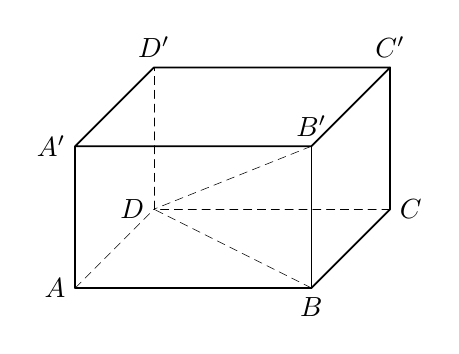
\begin{tikzpicture}[>=latex,scale=1.0]
  \tkzDefPoints{0/0/A,3/0/B,4/1/C,1/1/D,0/1.8/A'}
  \tkzDefPointsBy[translation=from A to A'](B,C,D){B',C',D'}
  \tkzDrawPolygon[semithick](A',B',C',D')
  \tkzDrawSegments[densely dashed](A,D C,D D,D' B',D B,D)
  \tkzDrawSegments[semithick](A,A' B,B' C,C' A,B B,C)
  \tkzLabelPoints(B)
  \tkzLabelPoints[left](A,A',D)
  \tkzLabelPoints[right](C)
  \tkzLabelPoints[above](D',B',C')
\end{tikzpicture}
\end{document}